\documentclass[a4paper,11pt]{article}
\usepackage{times}

\usepackage[top=1in, bottom=1in, left=0.5in, right=0.5in]{geometry}
\usepackage{graphicx}
\usepackage{wrapfig}
\usepackage{amsmath}
\usepackage{url}
\usepackage{units}

\begin{document}

\date{February 27, 2014}

\title{Elevator}

\author{Roshan.R\\
120050082\\
\texttt{roshanr@cse.iitb.ac.in}\\
\and Aakash Deshpande\\
120050005\\
\texttt{aakashd@cse.iitb.ac.in}\\
\and Deepak Verma\\
120050012\\
\texttt{deepakkota@cse.iitb.ac.in}}

\maketitle

\section{A Mechanical Elevator}

With sturdy metal beams as their building blocks, architects and engineers could erect monumental skyscrapers hundreds of feet in the air. But these towers would have been basically unusable if it weren't for another technological innovation that came along around the same time. Modern elevators are the crucial element that makes it practical to live and work dozens of stories above ground. Even in smaller multi-story buildings, elevators are essential for making offices and apartments accessible to handicapped people.

But this did not make elevators popular or worthwile. In 1853, American inventor Elisha Otis demonstrated a freight elevator equipped with a safety device to prevent falling in case a supporting cable should break. This increased public confidence in such devices. In 1853, Elisha Otis established a company for manufacturing elevators and patented (1861) a steam elevator. While, Elisha Graves Otis did not actually invent the first elevator, he did invent the brake used in modern elevators, and his brakes made skyscrapers a practical reality. His design was a purely mechanical masterpiece.\\

We have aimed to replicate this original design not just in essence, but with all the elements which made it viable.
In this project we have not just explained how these ubiquitous machines move you from floor to floor. We have aimed to create a realistic and practical instance of a working machine that can be deployed for use. For this, we'll also look at the control systems that decide where the elevator goes and the safety systems that prevent catastrophes.	

We have aimed to replicate this original design not just in essence, but with all the elements which made it viable.
In this project we have not just explained how these ubiquitous machines move you from floor to floor. We have aimed to create a realistic and practical instance of a working machine that can be deployed for use. For this, we'll also look at the control systems that decide where the elevator goes and the safety systems that prevent catastrophes.	

We have aimed to simulate an entirely mechanical device, that does not rely on artificial external forces or impulses. We have wrapped this in a package by creating a simple user interface similar to one in an ordinary elevator. 

We promised to develop a fully self-suffecient working model of an Elevator which could perform all basic functions of the elevator. We have done this using the following parts.

\subsection{Rope and counterweight}

The most popular elevator design is the roped elevator. In roped elevators, the car is raised and lowered by traction steel ropes rather than pushed from below. The ropes that lift the car are also connected to a counterweight, which hangs on the other side of the sheave. 
We have wrapped the elevator box and counterweight in two frames which constrain the bodies to move in a particular direction only.
These frames allow the elevator to rest exactly on particular floors, and move vertically at manageable speeds. The counterweight has been carefully chosen to balance the weight.

** Our working model consists of an elevator bound to a counterweight using not one, but a dual pulley joint. However, the pulleys are not connected directly to the elevator box, but a aseries of safety latches. Connecting the pulley to these safety devices allows them to react to changes in the state of the pulley or counterweight.


\begin{center}
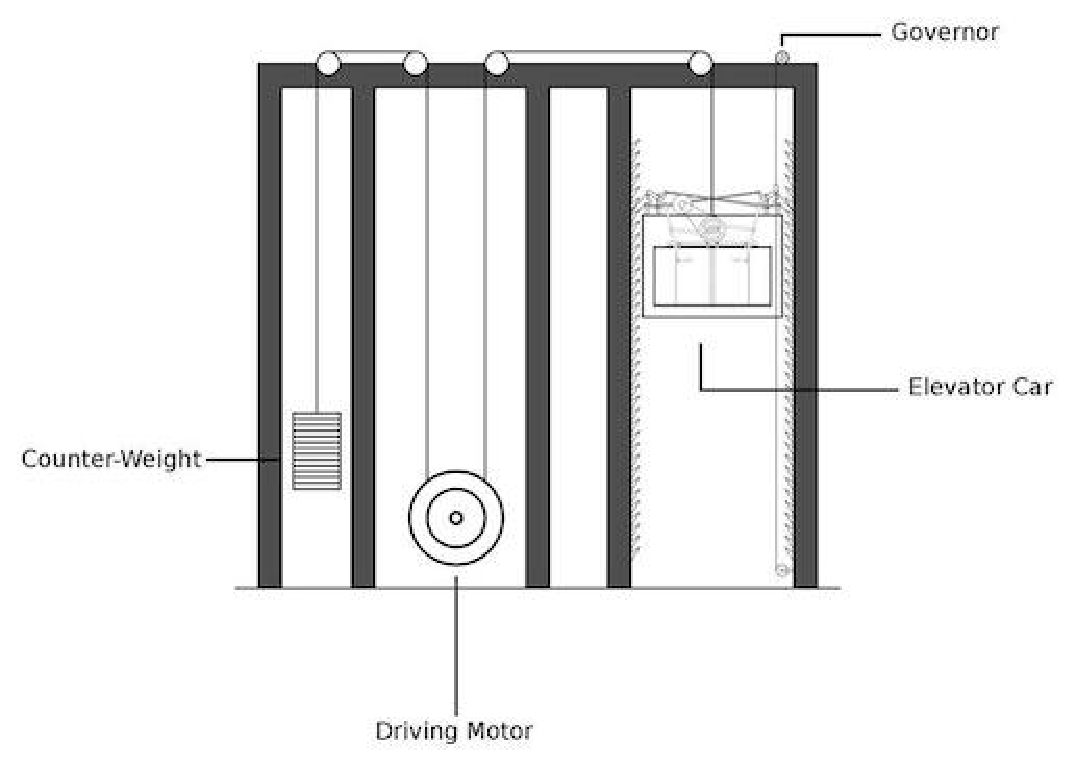
\includegraphics[width=0.6\textwidth]{images/elevatorOrig.eps} 
\end{center}


\begin{center}
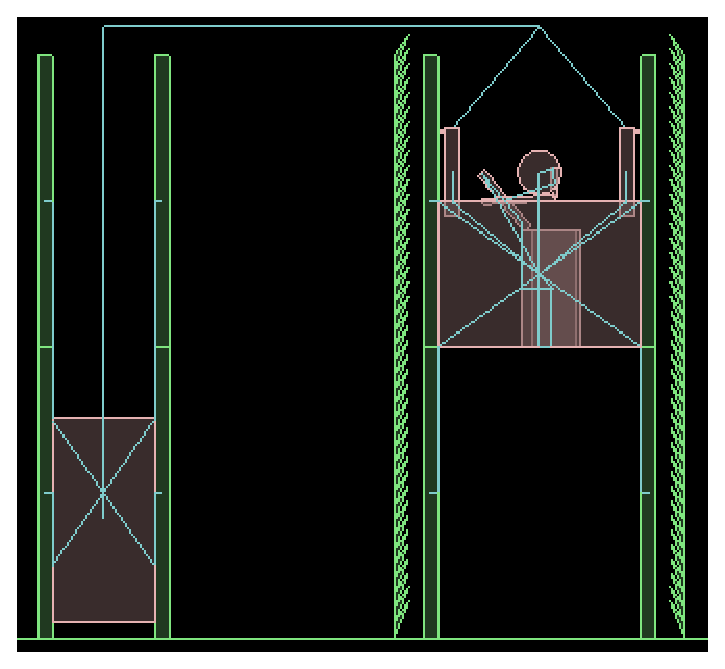
\includegraphics[width=0.6\textwidth]{images/elevator.eps} 
\end{center}

Our rope and pulley system has been designed as stated in the design. We have removed a few superfluous bars which are unescessary as Box2D can fix an object at anny point in the frame. For the driving motor, we have used the only motor inherently present in Box2D, the motor linked to a joint.

\subsection{Safety measures}

Proper safety measures are essential to make the elevator practical. We have created a braking system for the same.

The first line of defense is the rope system itself. Each elevator rope is made from several lengths of steel material wound around one another. With this sturdy structure, one rope can support the weight of the elevator car and the counterweight on its own. But elevators are built with multiple ropes (between four and eight, typically). In the unlikely event that one of the ropes snaps, the rest will hold the elevator up.

Even if all of the ropes were to break, or the sheave system were to release them, it is unlikely that an elevator car would fall to the bottom of the shaft. Roped elevator cars have built-in braking systems, or safeties, that grab onto the rail when the car moves too fast.
** Our working model consists of an extra frame of spikes and latches which form the braking system for the elevator in case the thread is cut. These latches are connected to the pulley and react to the tension in the thread to immediately snap open and lock the elevator in case of any mishap. Again, we have accomplished this using entirely mechanical parts without applying any external force.

As you can see in our design, this safety mechanism has been placed at the top of the elevator with the same working principle as Elisha Otis design.

\begin{center}
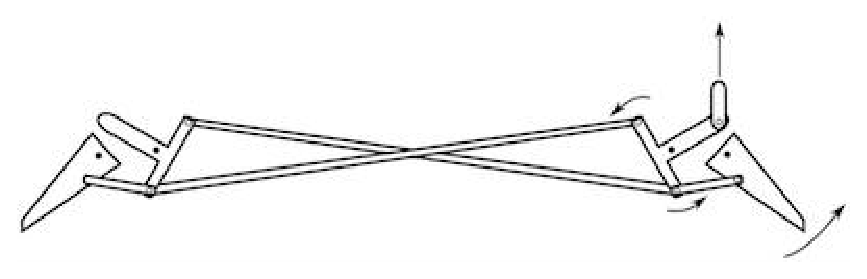
\includegraphics[width=0.6\textwidth]{images/safetyOrig.eps} 
\end{center}


\begin{center}
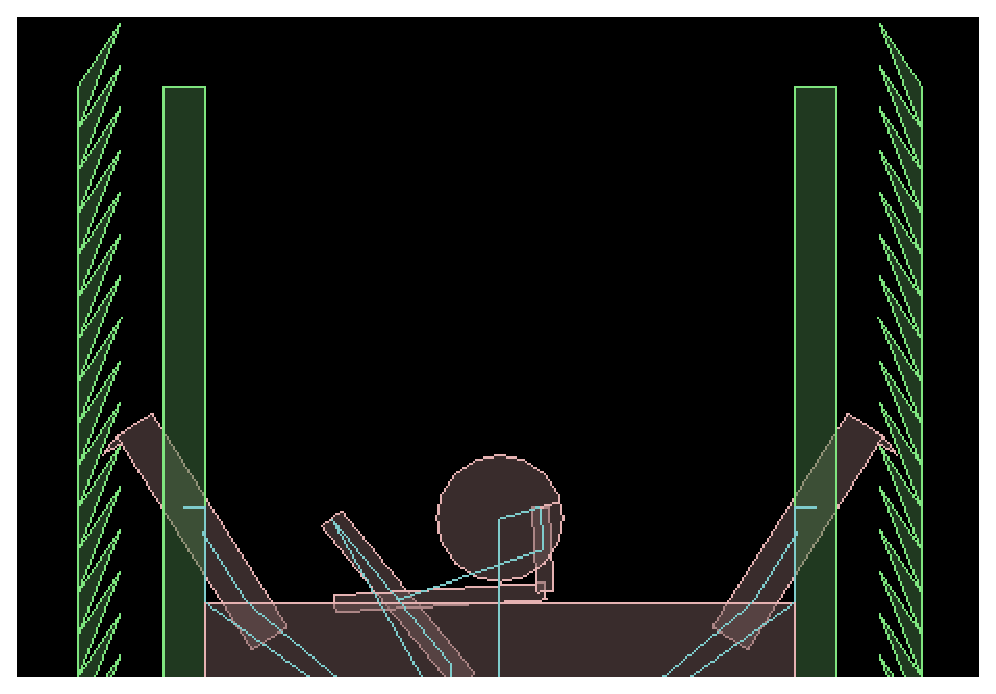
\includegraphics[width=0.6\textwidth]{images/safety.eps} 
\end{center}

\subsection{Elevator doors}

The automatic doors in an elevator are absolutely essential. They are there to keep people from falling down an open shaft.
The electric motor turns a wheel, which is attached to a long metal arm. The metal arm is linked to another arm, which is attached to the door. The door can slide back and forth on a metal rail.

When the motor turns the wheel, it rotates the first metal arm, which pulls the second metal arm and the attached door to the left. 

** Our model ensures that elevator doors open only when the elevator has reached a particular floor. Further, it locks down the elevator box to ensure that there is no movement or vibration while the doors are opening. Also, the doors remain closed when the elevator is moving vertically. The elevator cannot be stopped and the doors cannot be opened in the middle of the simulation 

We have replicated the sliding door model exactly as used in modern day elevators, complete with a wheel and rod system. However, as our simulation is 2-dimensional and the space on top of the elevator is constrained, we have done the same using one door. agin, we have replaced the motor with a joint motor as in Box2D.

\begin{center}
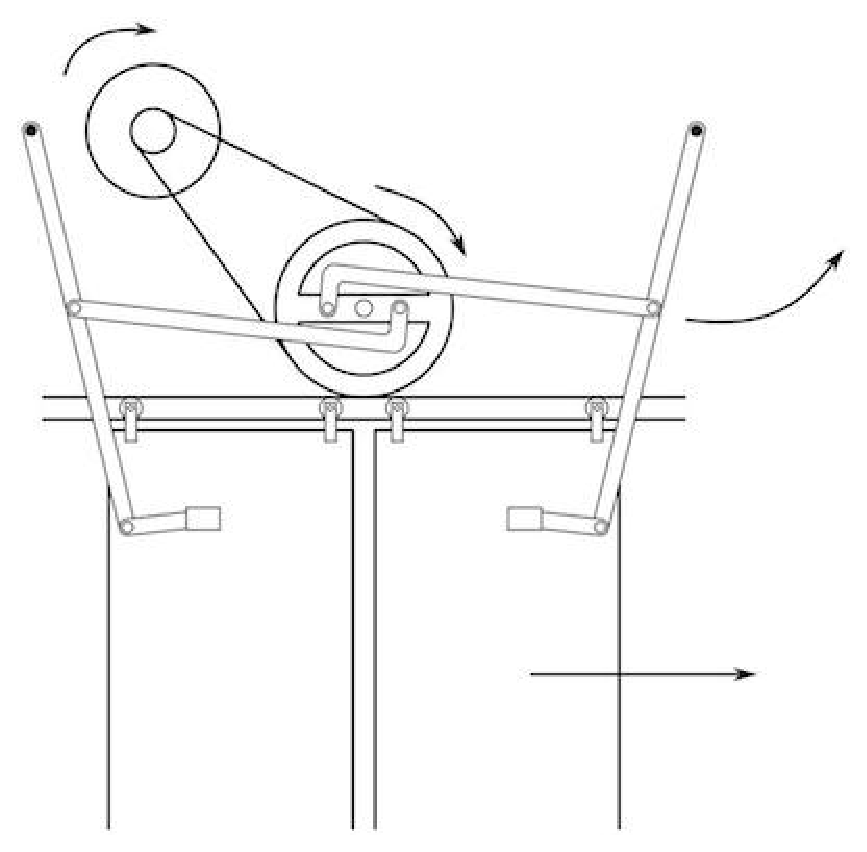
\includegraphics[width=0.6\textwidth]{images/doorOrig.eps} 
\end{center}


\begin{center}
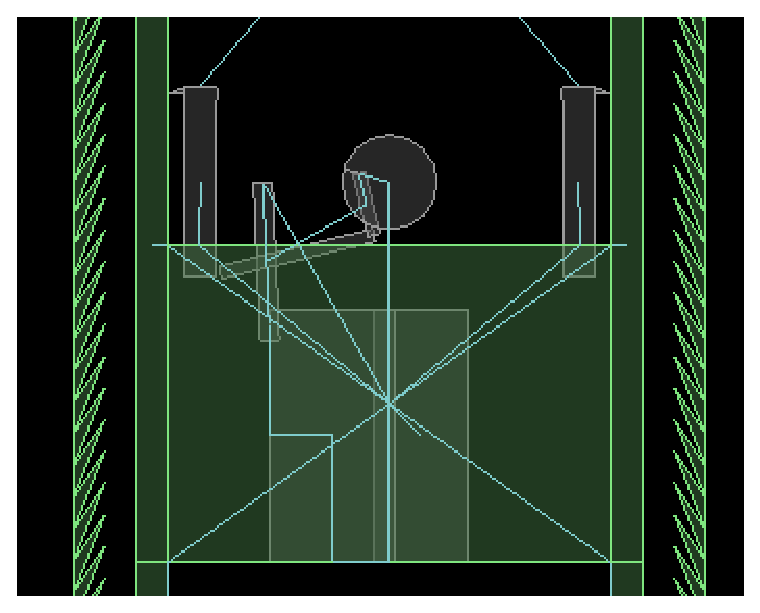
\includegraphics[width=0.6\textwidth]{images/door.eps} 
\end{center}

\subsection{Working and controls}

We have an interface consisting of an instruction set and certain keyboard buttons.
Instructions are as follows:

\begin{tabular}{l l l}
& 1. & d: Lift descends to the lower level, if there is any, and the doors get locked. This works only if the doors are closed. \\
& 2. & a: Lift ascends to the just higher level and the doors get locked. This works only if the doors are closed. \\
& 3. & l: Lift gets locked in position and the door slides opens. This will occur only if the lift is at some floor.\\
& 4. & c: Caution. The elevator thread gets cut!\\

\end{tabular}

A major challenge in our project was to increase the stability of the system. The elevator and counterweight used to bounce violently when the elevator stopped after some motion. Also, the safety mechanism gave a violent jerk when we suddenly applied a powerful brake to the system. We prevented this by constraining the motion of the machine using joint limits and by varying the weights of the different bodies involved.

Also, there is a computer system involved in most elevators which controls the movement of the machine. For example, the elevator box must precisely stop at a particular floor and not in between. 

In a relatively short period of time, elevators have become an essential machine. As people continue to erect monumental skyscrapers and more small buildings are made handicap-accessible, elevators will become an even more pervasive element in society. 

\section{Timing and profiling}
The following part of the report is an attempt to analyse and profile Box2D code written for Lab 05. We try to accomplish this using three methods to obtain data.

\begin{tabular}{l l l}
& 1. & Graphically plotting time using GNUplot\\
& 2. & Using profiling tools gprof and perf\\
& 3. & Using a call graph created using python script\\
\end{tabular}

\section{Graphically plotting time using GNUplot}
Timig and profiling our code was a challenge as our code behaves differently and responds to diferent keyboard commands. We overcame this by creating versions of our code which execute certain commands by default and then trying to put together the pieces by analysing all the seperate plots that we generated. This was done by making variables global and then imposing conditions on them inside the step function of the Box2D code. 

We plotted five graphs using data obtained from four functions of the code. The code was run for values of iteration ranging from 1 to 500 and the values were averaged over 15 reruns for each iteration value. Here are our observations based on individual graphs. 

\subsection{Average step time and Loop time vs Iteration values}

\begin{center}
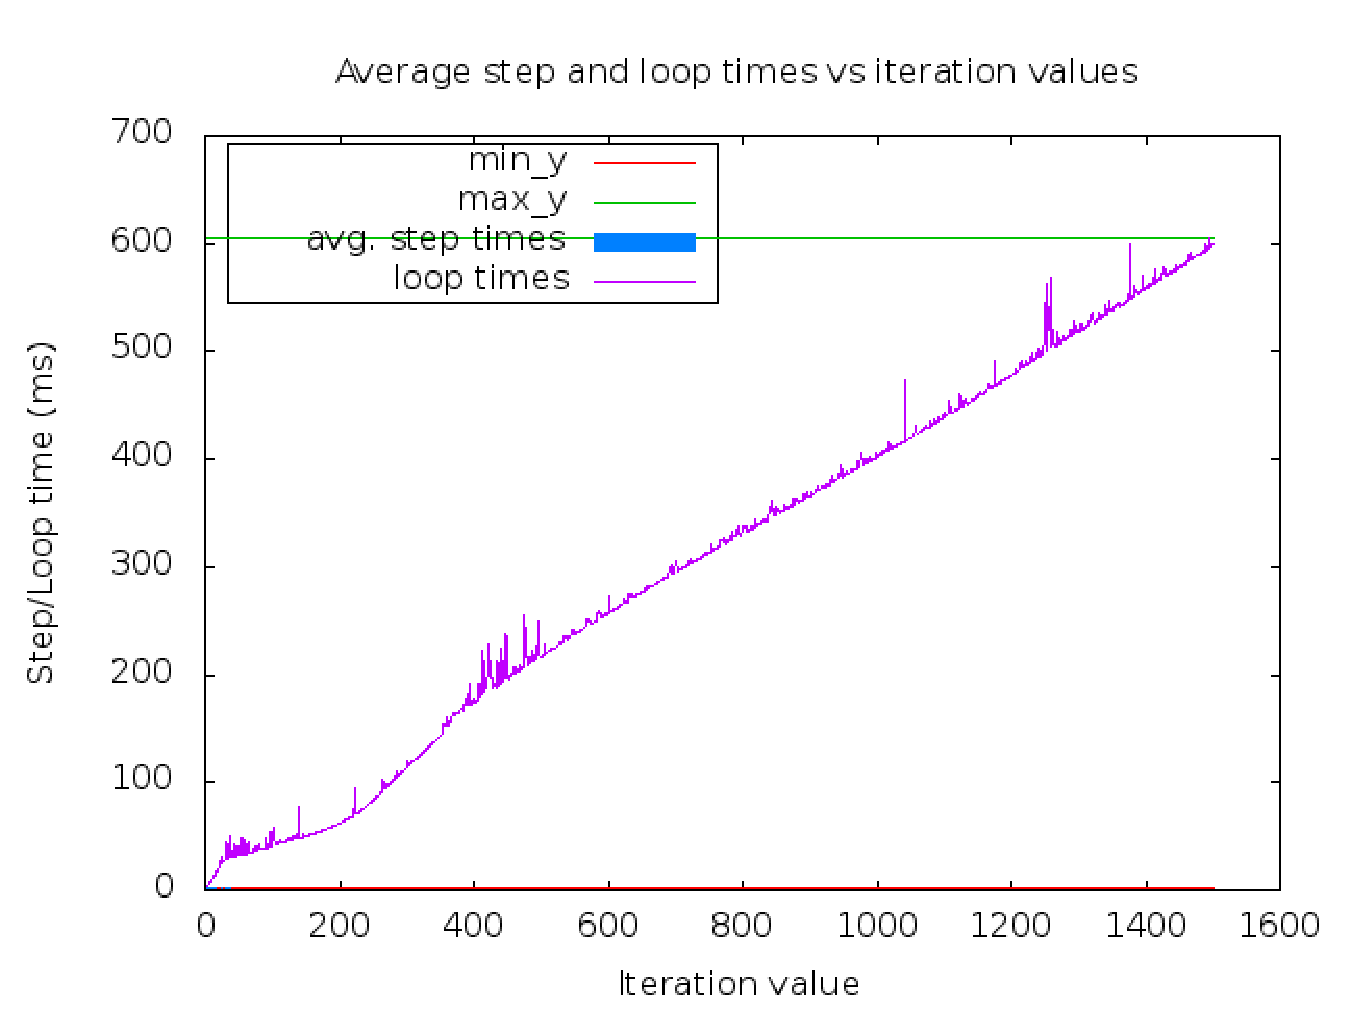
\includegraphics[width=0.6\textwidth]{plots/g05_plot01.eps} 
\end{center}

The histogram of the average step time shows that the average step times decrease continuously with increase in number of iteration values.This implies that the later steps take lesser aount of time as compared to the initial few iterations. this is consistent with our expectations as the earlier steps involve declaration and initialisation of a large number of objects.
The average step times are dominated by the loop times. The total loop times increase almost linearly with iteration values. As the individual loop times are in the same range, the cumulative or total loop times are continuous and linearly increasing.   

\subsection{Average step time and collision, velocity, position update time vs Iteration values}

\begin{center}
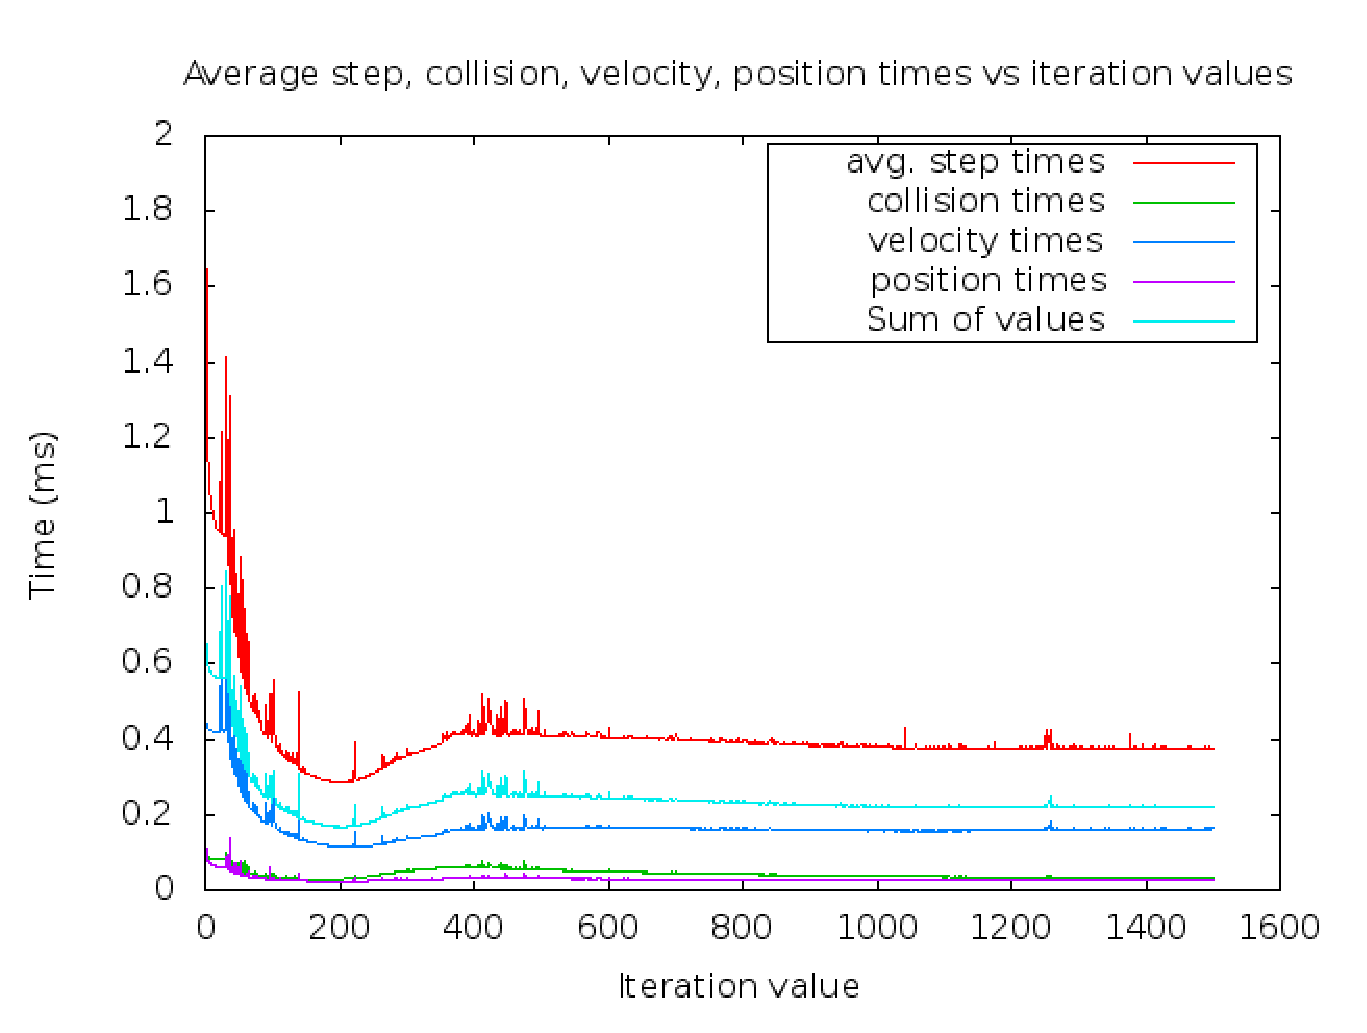
\includegraphics[width=0.6\textwidth]{plots/g05_plot02.eps} 
\end{center}

This is a line graph used for comparison between the different functions involved in one iteration. We can see the relationship between step, collision update, position update, velocity update functions of the dominos\_t created by the user. 

\begin{itemize}
  \item Step takes the maximum amount of time. In fact, it takes more time than the other three functions combined!
  \item Position and velocity calculations take almost the same amount of time, with velocity calculations taking marginally more time. 
  \item The points to note in this graph are the collision times which are almost zero. This is good news and desired as our simulation aims to create a smooth working machine with minimum collisions and greater effeciency. Higher average collision values would mean that our setup was wasting time on unnessecary calculations and our arrangement was not optimal.   

\end{itemize}

All the functions follow the same general pattern. The average times decrease steeply with increase in iteration values initially. Later, the average times settle down to almost constant values. 

There is a dip around the iteration value 200. The shape of the average values will depend on the simulation. For example, at the 200'th iteration, there might be a collision in the simulation. this will lead to an increase in moving parts and increase in calculations.\\

There are spikes in the graph representing anomalies. These are bad iterations. These spikes decrease in intensity with increase in iteration values as the anomalies get averaged out. 


\subsection{Average step time and error bars vs Iteration values}

\begin{center}
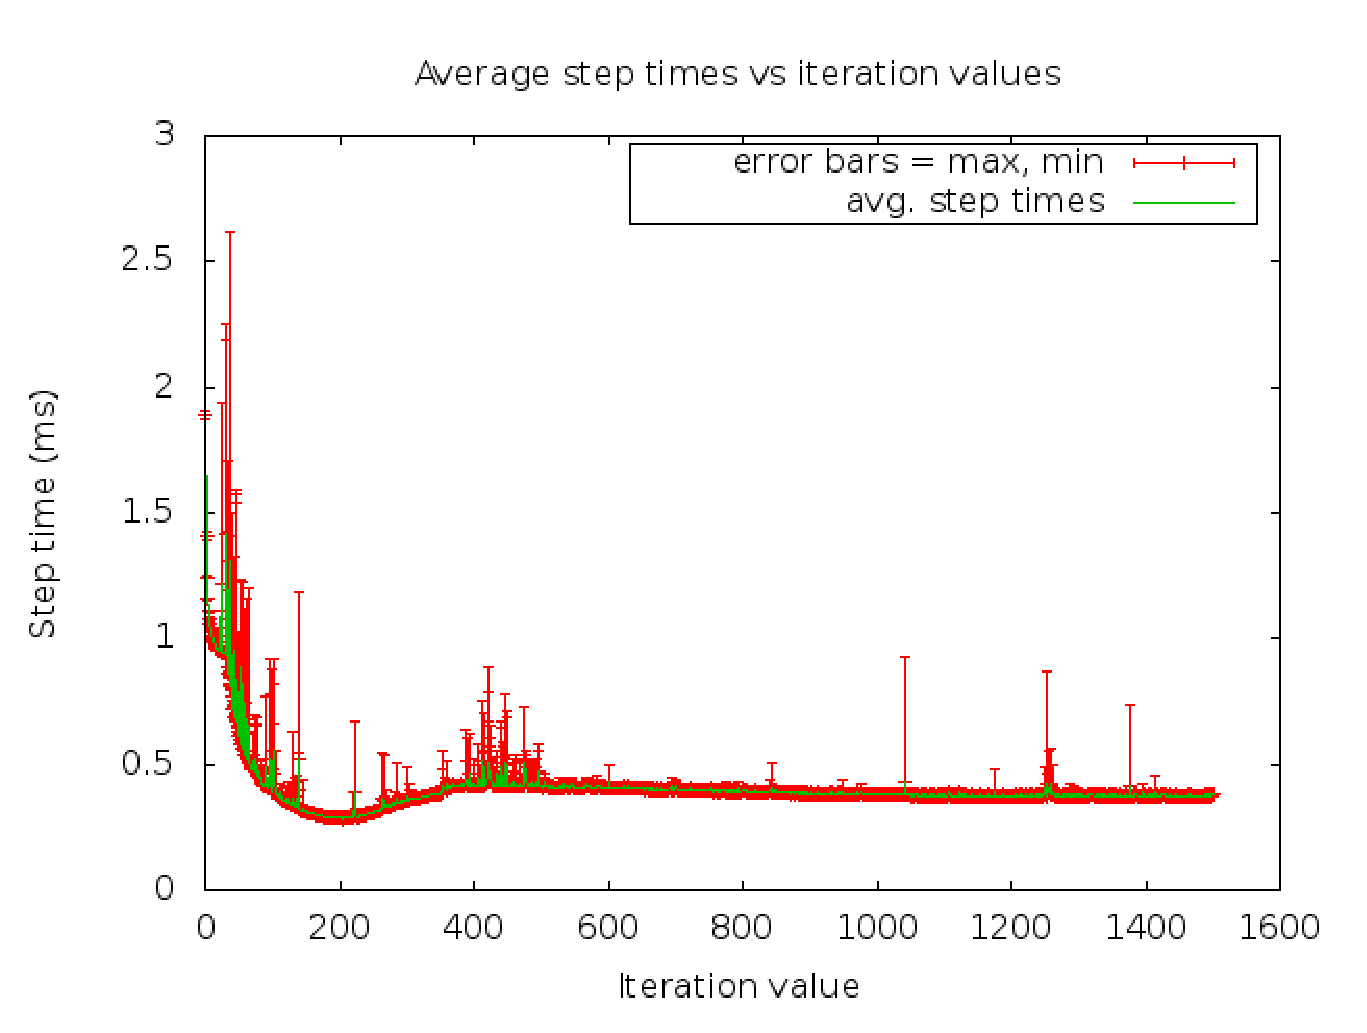
\includegraphics[width=0.6\textwidth]{plots/g05_plot03.eps} 
\end{center}

This graph shows the unpredictability of the time required for the system to execute various functions. The same function on the same hardware may take significantly different times when executed a second time. Thus we have error bars which vary upto a considerable distance from the average.

A significant trend is that anamolous points tend to take higher rather than lower values of time for execution. This error occurs because of the external load on the system due to other processes running parellely. But it is great news that most values of the average step times are in the lower end of the spectrum!

\subsection{Average step time over all values and over random values vs Iteration values}

\begin{center}
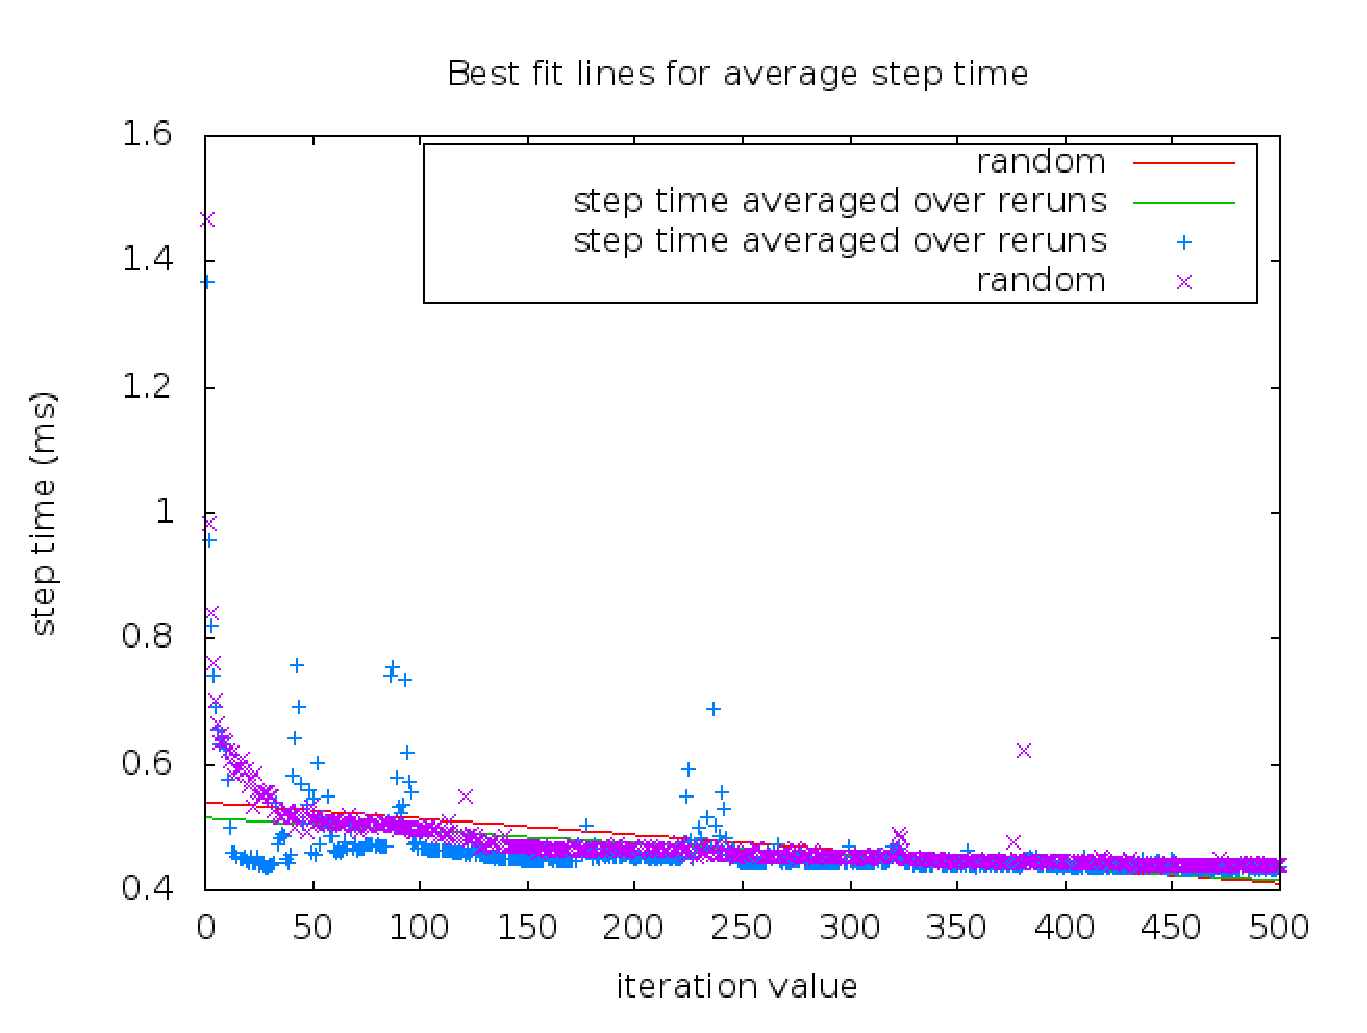
\includegraphics[width=0.6\textwidth]{plots/g05_plot05.eps} 
\end{center}

The best fit lines of the random and total values denote the closeness between the two values. Contrary to the earlier graph, this graph highlights the predictability of the step times. We have taken 10 random values out of a possible 15 and that can simulate the system to a high degree of accuracy.

\section{Analysing the effect of system processes}

The execution time depends a lot on the oher processes running on the system. These can be classified as memory intensive and CPU intensive processes. We tried the smulation with Firefox running. Firefox is notoriously memory intensive (it eats up about 1/5th of my RAM on average!). Naturally, the execution time increased by a few milliseconds. 
My sample execution over 10000 iterations of the code resulted in a total loop time of 1056.6 ms without Firefox and 1068.4 ms with it. The details are given later.

\section{Measuring time taken by the program to run}

The time command measures the whole program execution time, including the time it takes for the system to load the binary and all its libraries, and the time it takes to clean up everything once the program is finished.

On the other hand, gettimeofday can only work inside the program, that is after it has finished loading (for the initial measurement), and before it is cleaned up (for the final measurement).

Thus, the time and gettimeofday commands rerturn different times for execution, with time reporting a considerably larger nterval for execution.
If you are trying to time something in seconds, then time() is probably your best bet. If you need higher resolution than that, then I would consider gettimeofday(), which gives up to microsecond resolution (1 / 1000000th of a second).

\section{Profiling Code}

The code was run for 10000 iterations and profiled using gprof/perf. A call graph was also generated using gprof2dot.py python script and dot. Choosing large number of iterations means the program runs for enough time to generate meaningful data.

Also for small number of iterations, the average step time is high since some functions run for constant time(like initialisation of the world, etc). Therefore, by choosing large number of iterations, the contribution of these functions become negligible and the average step time remains fairly constant. This is also evident from the graph in the previous section.\\

\subsection{Debug option}
\begin{center}
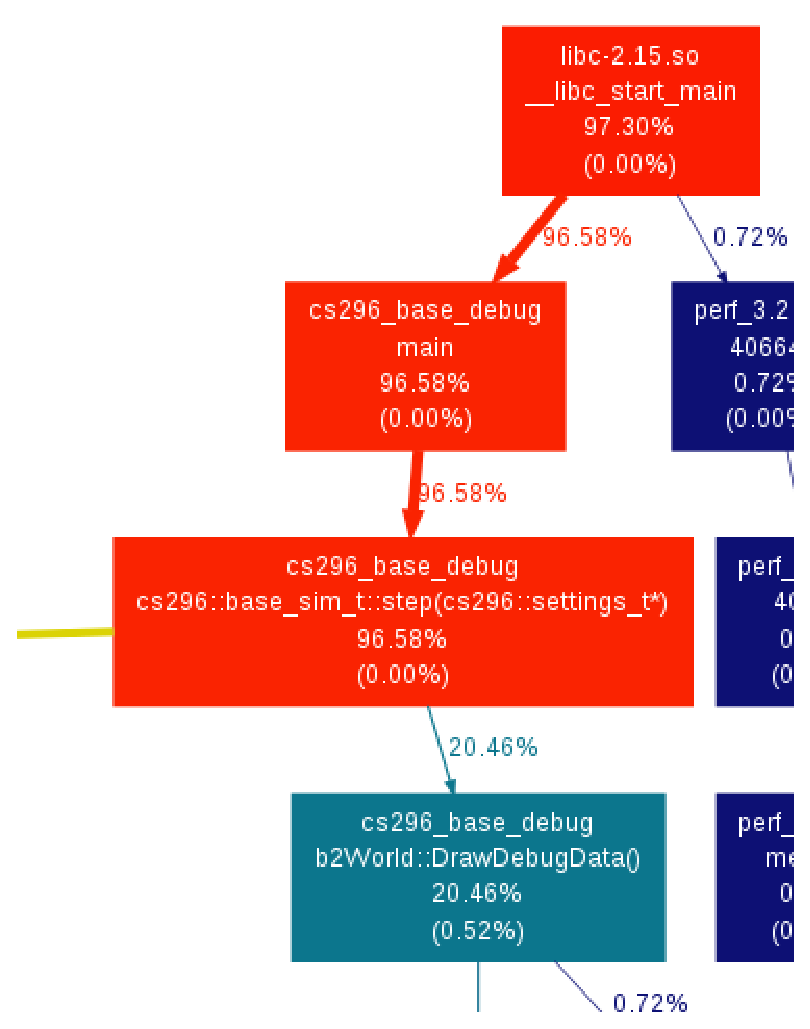
\includegraphics[width=0.4\textwidth]{images/debug1.eps}
\end{center}

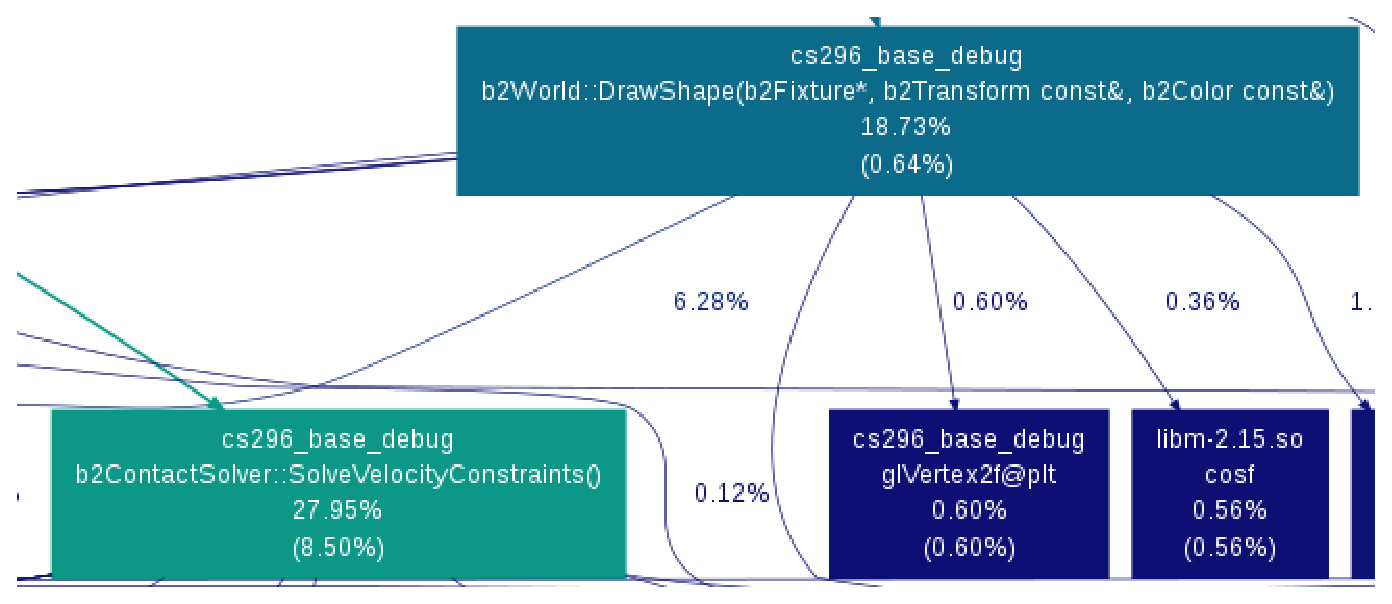
\includegraphics[width=0.4\textwidth]{images/debug3.eps}
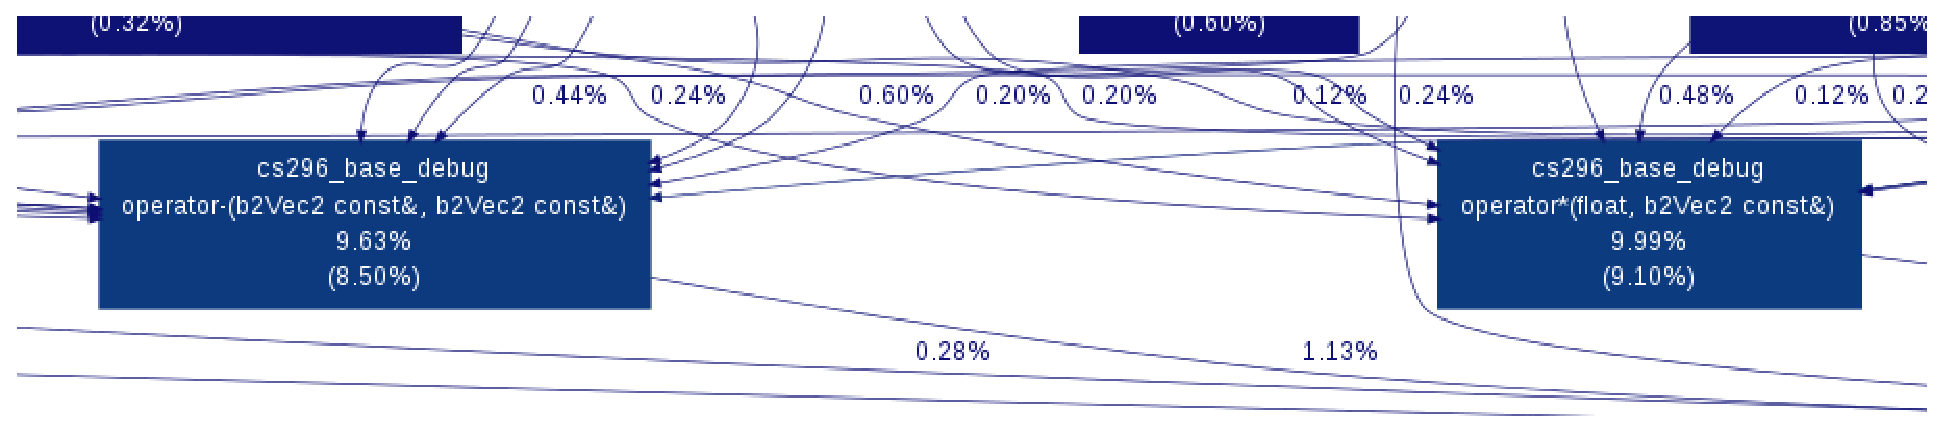
\includegraphics[width=0.55\textwidth]{images/debug2.eps}


When profiling using debug option, the total time taken is quite large. The number of function calls made are also high. There is no optimisation of the code done by the compiler. There is a single entry point through the main program which takes up most of the time.\\

\subsection{Release option}
\includegraphics[width=0.9\textwidth]{images/release.eps}
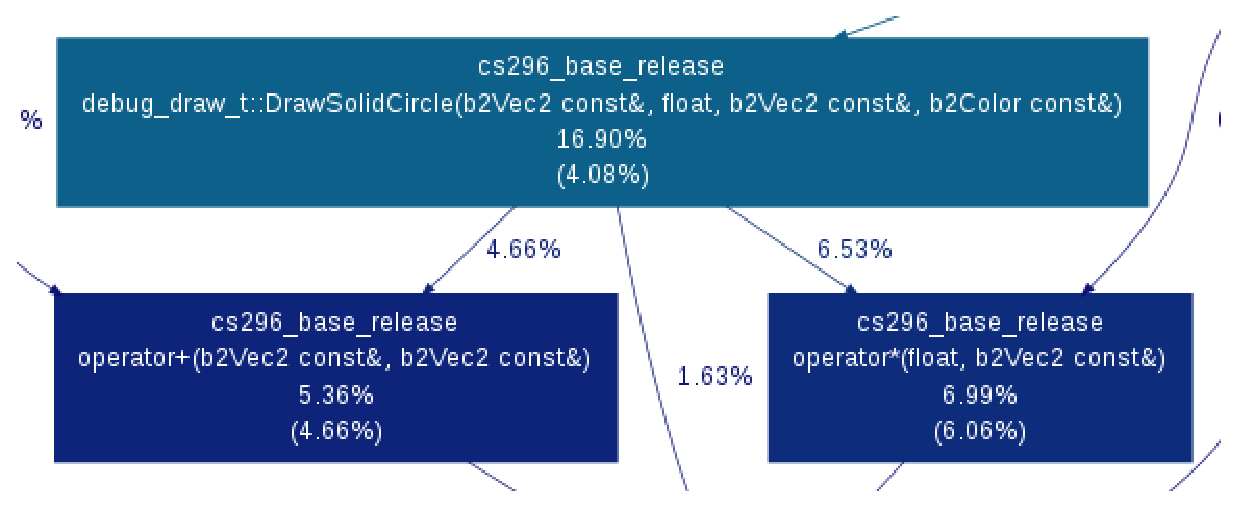
\includegraphics[width=0.4\textwidth]{images/release1.eps}
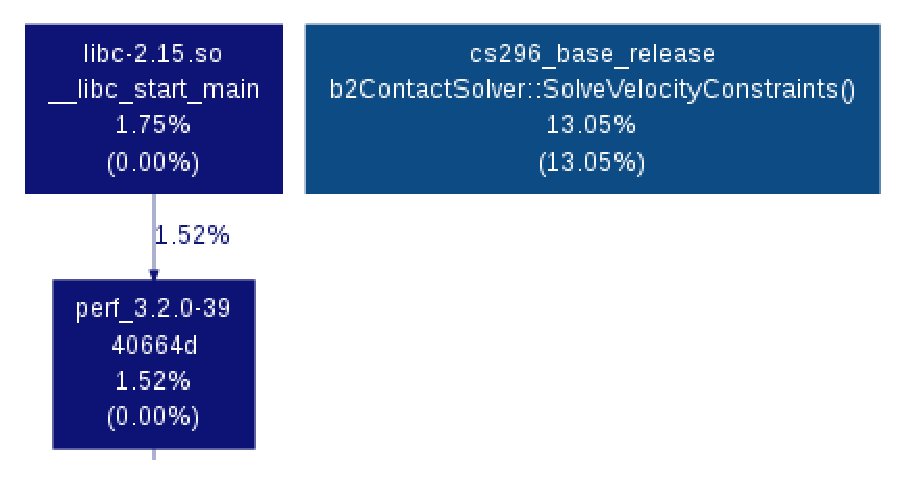
\includegraphics[width=0.5\textwidth]{images/release2.eps}


When profiling using release option, a lot lesser time was taken for execution. Also, lesser function calls were made. Since the code is compiled and built with -O3 flag, the code is heavily optimised by the compiler using things like aggressive loop unrolling and inlining of functions. There is a large space tradeoff to reduce function calls. Also, there is no single entry point suggesting that some kind of parallel optimisation is also taking place.

\subsection{Analysis}
As you can see, in both of them, most of the time is spent in doing math operations on Box2D vectors and solving the position/velocity constraints in the system induced by contacts and joints but the total number of function calls. The math operations are mainly used in drawing shapes.
Also, a lot of time is used by the libm math library which is fairly obvious given that basic math operations are used in all of the above tasks.

The time taken by the release build is three to four times the time taken by the debug build. Here is a sample of the code executed first as a release build and then as a debug build. The times vary substantially.

\subsection{Optimisation}
Due to the difference in debug and release times we see that certain functions can be made more effecient.
From the graph we observed that, the following functions take up lot of time and can possibly be optimized:

\begin{enumerate}
\item DrawShape()
\item SolveVelocityConstraints()
\item operator+()
\item operator-()
\item operator*()
\end{enumerate}

The big indicator of effeciency for our code are the collision times in the simulation. Our project required that the device be smooth and to not have unneseccary collisions. We went about this in the folllowing manner :

1. Better use of joints. 
The frame of the elevator and counterweight that we have designed can by itself support and maintain the elevator box in a vertical position. However, it was leading to wastefdul calculations. We added a prismatic joint to both these frames and reduced the number of collisions. 
A major block in the simulation is that the elevator box used to bounce or vibrate after we tried to hold it still on reaching a particular floor. We realised that fixing the elevator using a collision with another body was not a great idea as Box2D would involve itself in complex force and position calculations. Further, due to the timestep of the Box2D step function, the parameters after a collision are approximated to some degree. We observed that using the limits of a prismatic joint handled this job far better. 

2. Reducing unecessary bodies
Some bodies become irrelevant in a Box2D simulation as they can be replaced by Box2D feature. For example a motor can be replaced by the motor of a joint. Also, a rod holding together two objects can be replaced by a weld joint. We have tried to reduce the superfluous elements in our simulation.

3. Setting proper parameter values
We noted that Box2D could not easily handle bodies with very low densities. Their behavior with respect to joints and collisions was not proper and led to wild swings in behavior. This increased our calculations as the system oscillated violently about some wrong value. Also, the collisions in Box2D were not completely inelastic. This meant that the simulation took a lot of calculations to get to the rest stae. We modified the values of our parameters, for example, we scales up our body masses or scaled down our distances to reduce the perturbations in the system. 

To optimise it further, the constraint solving module of the Box2D library can be improved. Better equations and asynchronous procedures can be devised to reduce the time required to solve constraints/collisions. The math operations on vectors can be improved by making use of parallelisation features like SIMD. Also, some computation can be moved to the GPU and run parallel to the CPU.

\nocite{*}

\bibliographystyle{plain}
\bibliography{bibtex}

\end{document}
